\chapter{シグナル}

%==============================================================================
前の章では,
プロセスを終了させたり一時停止させたりするために
シグナルが利用できることを学んだ.
シグナルは動作中のプロセスに非同期的に(いつでも関係なく)
イベントの発生を知らせる汎用的な仕組みである.
JOB制御やアプリケーションの強制終了,
サーバプロセスの再起動などに使用される.

%==============================================================================
\section{シグナルの特徴と使用目的}
シグナルは,プロセスにイベントの発生を知らせるソフトウェア割り込みである.
割込みのようなものであるから,
プロセスはシグナルがいつ発生するか予測できない.
シグナルは以下のような場合にイベントをプロセスに通知するために使用される.

\begin{enumerate}
\item \emph{プロセスやOSがプロセスにイベントを通知する場合}\\
  kill コマンドを用いてシグナルをプロセスに送信する場合が一つの例である.
  kill コマンドの実行は,
  kill プログラムがプロセスとして実行されるのであるから,
  kill プロセスから目的のプロセスにシグナルを送っていることになる.

  もう一つの例はターミナルで Ctrl-C や Ctrl-Z を押した場合である.
  この場合はOSがターミナルに属するフォアグラウンドプロセスにシグナルを送る.

\item \emph{プロセス自身の異常を通知する場合}\\
  0での割り算を実行したり
  \footnote{Floating point exception シグナル(\texttt{SIGFPE})が発生する.}
  ,ポインタの初期化をし忘れて異常なアドレスをアクセスしたり
  \footnote{Segmentation fault シグナル(\texttt{SIGSEG})が発生する.}
  したことをプロセス自身に通知する.
  通常,この通知を受取るとプロセスは終了する
  \footnote{終了時に「\texttt{Segmentation fault: 11}」等が表示される.}

\item \emph{プロセスが予約した時刻になった場合}\\
  プロセスは一定時間後にシグナルを発生するように予約できる.
  時間になるとアラームシグナル(\texttt{SIGALRM})が発生する.
\end{enumerate}

%==============================================================================
\section{シグナル一覧}
よく使用するシグナルの一覧を\tabref{signal}に示す.
本当は1番から31番までのシグナルがあるが,
よく使用されるものだけを掲載する\footnote{
詳しくはオンラインマニュアル(\texttt{man 3 signal})を読むこと.}.
記号名はC言語のプログラムで使用できるシグナルの名前である.
デフォルトは,次の節で説明するシグナルハンドリングの初期状態を表す.
\texttt{SIGKILL}と\texttt{SIGSTOP}は\emph{ハンドリングを変更できない}.

\begin{mytable}{btp}{よく使用されるシグナルの一覧}{signal}
  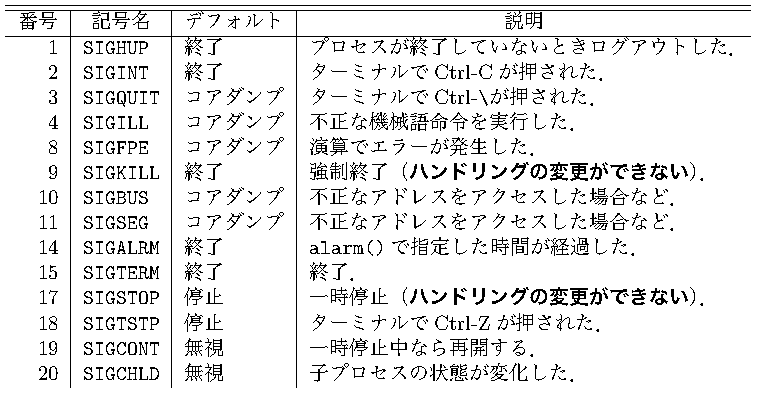
\includegraphics[scale=1.0]{Tbl/signal.pdf}
\end{mytable}

%==============================================================================
\section{シグナルハンドリング}
受け取ったシグナルをプロセスがどのように扱うかを
\emph{シグナルハンドリング}と言う.
シグナルハンドリングは,
次の節で紹介するsignalシステムコールを用いて,
プロセス自身がシグナルの種類ごとに予め決めておく.
指定できるシグナルハンドリングは以下の三種類である.

\begin{enumerate}
\item \emph{無視(ignore)}
  そのシグナルを無視する.

\item \emph{捕捉・キャッチ(catch)}
  そのシグナルを受信し,
  登録しておいたシグナル処理ルーチン(シグナルハンドラ関数)を呼び出す.

\item \emph{デフォルト(default)}
  シグナルの種類ごとに決められている初期のハンドリングであり,
  以下の四種類のどれかである.
  各シグナルのデフォルトが四種類のうちのどれかは\tabref{signal}から分かる.
  %例えばデフォルト状態のまま
  %\texttt{SIGHUP}シグナルを受信するとプロセスは終了するし,
  %\texttt{SIGTSTP}シグナルを受信するとプロセスは停止する.

  \begin{description}
  \item[停止] プロセスは一時停止状態になる.
  \item[無視] プロセスはそのシグナルを無視する.
  \item[終了] プロセスは終了する.
  \item[コアダンプ] プロセスはcoreファイル
    \footnote{プロセスのメモリイメージを書き出したファイルのこと.
      デバッグに使用することができる.
      macOSの標準ではコアダンプしても
      コアファイルを作らないように設定されている.}
    を作成してから終了する.
  \end{description}
\end{enumerate}

%==============================================================================
\section{signalシステムコール}
自プロセスのシグナルハンドリングは signal システムコール\footnote{
  最近のUNIXやmacOSではsignalはライブラリ関数である.
  しかし,古いUNIXではシステムコールだったので,
  ここでは「signalシステムコール」と呼ぶ.}
を使用して変更できる.

\begin{description}
\item[書式] 次の通りである.
\begin{lstlisting}[numbers=none]
  #include <signal.h>
  sig_t signal(int sig, sig_t func);
\end{lstlisting}

\item[解説]
  signalシステムコールは,
  自プロセスの指定されたシグナルのハンドリングを変更する.
  \|sig_t|型は関数ポインタ型\footnote{
    関数のアドレスを表す型である.
  }であり,\texttt{signal.h}をインクルードすることで自動的に宣言される.

\item[引数]
  第1引数(\texttt{sig})はハンドリングを変更するシグナルの種類である.
  種類は\tabref{signal}に示した番号または記号名で指定する.
  第2引数(\texttt{func})は新しいハンドリングである.
  以下の3種類から一つを指定する.

  \begin{enumerate}
  \item \texttt{SIG\_IGN}はシグナルを無視するようにする.
  \item \texttt{SIG\_DFL}はシグナルハンドリングをデフォルトに戻す.
  \item \emph{シグナルハンドラ関数}を指定する\footnote{
    関数の名前を書けばよい.C言語で関数名は関数を指すポインタになる.}と,
    そのシグナルを捕捉(キャッチ)できるようになる.
    シグナルを捕捉した時にシグナルハンドラ関数が実行される.
    シグナルハンドラ関数の型は\|void func(int sig);|でなければならない.
    引数\texttt{sig}には捕捉したシグナルの番号が渡される.
  \end{enumerate}

\item[戻り値]
  正常なら変更前のハンドリングが返される.
  これを\texttt{sig\_t}型の変数に記録しておけば,
  後でハンドリングをもとに戻すことができる.
  エラーが発生した場合は\texttt{SIG\_ERR}が返され,
  \texttt{errno}変数にエラー番号がセットされる\footnote{
    後で\texttt{perror()}関数が\texttt{errno}変数を参照して,
    エラー原因を表示することができる.}.

\item[プログラム例] signalシステムコールを使用するプログラムの例を二つ示す.
  \begin{enumerate}
  \item \emph{シグナルを無視する例} \\
    リスト\ref{ignore}に\texttt{SIGINT}を一時的に無視するプログラムの例を示す.
    5行でCtrl-Cを無視するようにハンドリングを変更する.
    6行ではCtrl-Cを押してもプログラムが終了しない状態になっている.
    7行でハンドリングを元に戻しCtrl-Cで終了するようにする.

    \lstinputlisting[numbers=left,caption=シグナルを無視する例,
      label=ignore,float=btp]{Lst/signalIgnore.c}
    
  \item \emph{シグナルを捕捉する例} \\
    リスト\ref{catch}に\texttt{SIGINT}を捕捉するプログラムの例を示す.
    9行から11行の間を実行中は,
    Ctrl-Cが押される度に\texttt{handler()}関数が実行される.
  
    \lstinputlisting[numbers=left,caption=シグナルを補足する例,
      float=btp,label=catch]{Lst/signalCatch.c}
  \end{enumerate}

\end{description}

%==============================================================================
\section{シグナルハンドラの制約}
シグナルは割り込みのようなものなので,
ハンドラ関数はいつ呼び出されるか分からない.
そのためシグナルハンドラ中でやって良い処理には強い制約がある.
例えば\texttt{printf()}を実行している途中で
シグナルが発生した場合を考えて欲しい.
シグナルハンドラの内部で\texttt{printf()}関数を呼出したらどうなるだろうか.
何かまずいことが起こりそうな気がする.

\subsection{制約がある理由}
\texttt{printf()}関数を例に制約が必要な理由を考えてみよう.
\texttt{printf()}は高水準I/Oの関数なので出力する内容を一旦バッファに書き込む.
バッファに書き込む処理の最中にシグナルが発生し,
シグナルハンドラが呼出されたとする.

もしも,
シグナルハンドラ中に\texttt{printf()}の呼び出しが含まれていると,
新しい\texttt{printf()}も同じバッファに出力を書き込むので,
バッファのデータが壊れるかもしれない.
\texttt{printf()}に限らず多くのライブラリ関数は,
シグナルハンドラから呼び出されることを前提に設計されていない.

\subsection{やってもよいこと}
\texttt{printf()}関数の例では説明できなかった他の理由もあるので,
シグナルハンドラでは次の三つのことしかやってはならない.

\begin{enumerate}
\item シグナルハンドラ関数のローカル変数の操作
\item \texttt{volatile sig\_atomic\_t} 型変数の読み書き
  \footnote{\texttt{sig\_atomic\_t} 型はmacOSでは\texttt{int}型である.
    \texttt{volatile}を付けるとCコンパイラの最適化の対象外になる
           (詳細はコンパイラにより異なる.).
           コンパイラの最適化は変数がシグナルハンドラなどから非同期に
           アクセスされることを前提にしていない.
           更に注意が必要なことは,これらの制約がある上に「読み書き」が
           単純な\emph{参照}と\emph{代入}のことしか指していないことである
           (インクリメントが正しく動く保証はない.).}
\item 非同期シグナル安全な関数の呼び出し
\end{enumerate}

非同期シグナル安全な関数は,
例えば次のような関数(システムコールも含む)である\footnote{
詳細はオンラインマニュアル\texttt{man sigaction} を参照のこと.}.

\texttt{\_exit(), alarm(), chdir(), chmod(), close(), creat(), dup(),
dup2(), execle(), execve(), fork(), kill(), link(), lseek(), mkdir(),
open(), pause(), read(), rename(), rmdir(), signal(), sleep(), stat(),
time(), unlink(), wait(), write(), strcpy(), strcat(), ...}

%==============================================================================
\section{シグナルハンドラの例}
リスト\ref{handler}に Ctrl-C を三回押すまで終了しないプログラムの例を示す.
3行はシグナルハンドラから操作して良い変数\texttt{flg}を宣言している.
4行からがシグナルハンドラ関数である.
シグナルハンドラは\texttt{flg}の単純な代入と,
非同期シグナル安全な\texttt{write()}の実行しかしない.

\lstinputlisting[numbers=left,caption=シグナルハンドラの例,label=handler,
  float=btp]{Lst/signalHandler.c}

10行で\texttt{handler()}を\texttt{SIGINT}のハンドラ関数として登録している.
11行のwhile文で,変数\texttt{flg}が1になった回数を数えている.
\texttt{main()}でも\texttt{flg}は単純な\emph{参照}と\emph{代入}しかしない.
このように,ハンドラ関数ではフラグを立てることと,
安全なシステムコールの呼び出し程度のことしかできない.

%==============================================================================
\section{killシステムコール}
プロセスがプロセスにシグナルを送信するシステムコールである.

\begin{description}
\item[書式] 以下の通りである.
\begin{lstlisting}[numbers=none]
  #include <signal.h>
  int kill(pid_t pid, int sig);
\end{lstlisting}

\item[解説]
  killシステムコールは,
  送信先のプロセスとシグナルの種類を指定してシグナルを送信する.

\item[引数]
  第1引数(\texttt{pid})は送信先プロセスのプロセス番号である.
  \|pid_t|はプロセス番号を格納するのに都合の良い整数型である.
  第2引数(\texttt{sig})は送信するシグナルの種類である.
  種類は\tabref{signal}に示した記号名または番号で指定する.

\item[戻り値]
  正常時は0,異常時-1が返される.
  その際,エラー番号が\|errno|変数にセットされる.

\item[プログラム例]
  リスト\ref{kill}にkillシステムコールの使用例として,
  killコマンドを簡単化したプログラム(mykill)を示す.
  このプログラムは,シグナル番号とプロセス番号を引数に実行し,
  指定されたシグナルを指定されたプロセスに送信する.
  11,12行の\|atoi()|関数は,
  10進数を表す文字列(例えば\|"123"|)から整数値(int型の123)を
  求める関数である\footnote{
    詳しくはオンラインマニュアル\texttt{man 3 atoi}で調べること.}.
  リスト\ref{grapher}に,このプログラムの使用例を示す.

\lstinputlisting[numbers=left,caption=簡易killプログラム(mykill),
  float=btp,label=kill]{Lst/mykill.c}

\lstinputlisting[numbers=left,caption=簡易killプログラム(mykill)の実行例,
  label=grapher,numbers=none,float=btp]{Lst/mykill.txt}

\end{description}

%==============================================================================
\section{シグナルと合わせて使うシステムコール}

プロセスを待ち状態にするシステムコール\footnote{
本当はライブラリ関数であるが,
古いUNIXではシステムコールだったので,
ここではシステムコールと呼ぶ.}と,
シグナルを予約するシステムコールを紹介する.

\subsection{sleepシステムコール}
自プロセスを指定された時間,またはシグナルを受信するまで,
待ち状態にする.

\begin{description}
\item[書式] 以下の通りである.

\begin{lstlisting}[numbers=none]
  #include <unistd.h>
  unsigned int sleep(unsigned int seconds);
\end{lstlisting}

\item[解説]
  sleepシステムコールは時間を決めて自プロセスを待ち状態にする.
  もしも待ち状態になっている間にシグナルが届いた場合は,
  そのシグナルのハンドリングが\emph{無視以外}なら,
  待ち状態が解除される(sleepシステムコールが終了する.).
  シグナルを捕捉した場合は直ちにシグナルハンドラが実行される.

\item[引数]
  \texttt{seconds}は待ち時間を秒単位で指定する.

\item[戻り値]
  待ち時間が経過してsleepシステムコールが終了した場合は0が返される.
  シグナルで終了した場合はsleep予定だった残りの秒数が返される.
  
\item[プログラム例]
  リスト\ref{sleep}に1秒に一度\|hello|と表示するプログラムを示す.

  \lstinputlisting[caption=sleepシステムコールの使用例,language=C,
    float=btp,label=sleep]{Lst/sleep.c}

\end{description}

\subsection{pauseシステムコール}
時間制限がないsleepシステムコールである.

\begin{description}
\item[書式] 以下の通りである.

\begin{lstlisting}[numbers=none]
  #include <unistd.h>
  int pause(void);
\end{lstlisting}

\item[解説]
  pauseシステムコールはシグナルが到着するまでプロセスを待ち状態にする.
  シグナルを受信した時の動作はsleepシステムコールと同様である.
  シグナルを受信した時,
  ハンドリングが\emph{終了}になっている場合はプロセスが終了する.
  ハンドリングを\emph{捕捉}にしてから待たなければならない.

\item[戻り値]
  -1が返される.(常時エラー)\footnote{
    シグナルによってエラーが発生しpauseシステムコールが打ち切られた
    という意味である.
  }

\item[プログラム例]
  リスト\ref{pause}は
  シグナルが三回発生するのを pause システムコールで待つプログラムである.
  ハンドリングを捕捉にしていないと一回目のCtrl-Cでプログラムが終了するので,
  何もしないハンドラ関数を登録している.

  \lstinputlisting[caption=pauseシステムコールの使用例,language=C,
    float=btp,label=pause]{Lst/pause.c}

\end{description}

\subsection{alarmシステムコール}
アラームシグナルの発生を予約するシステムコールである.

\begin{description}
\item[書式] 以下の通りである.

\begin{lstlisting}[numbers=none]
  #include <unistd.h>
  unsigned int alarm(unsigned int seconds);
\end{lstlisting}

\item[解説]
  alarmシステムコールは
  \texttt{SIGALRM}シグナルが
  \texttt{seconds}秒後に発生するようにタイマーに予約をする.
  alarmシステムコールは予約するだけで待ち状態になる訳ではない.

\item[引数]
  \texttt{seconds}秒後にシグナルを発生する.
  0 を指定した場合は以前の予約を取り消す.

\item[戻り値]
  通常は0が返される.
  既に別の予約がされていた場合は前の予約の残り時間を返し,
  今回の\texttt{seconds}を用いてタイマーを再起動する.

\item[プログラム例]
  リスト\ref{alarm}は
  アラームシグナルが発生するまで
  pause システムコールで待つプログラムの例である.
  alarm システムコールはシグナルの予約をするだけなので,
  pause システムコールでプログラムを停止する.

  \lstinputlisting[caption=alarmシステムコールの使用例,language=C,
    float=btp,label=alarm]{Lst/signalAlarm.c}

\end{description}

\section*{課題 No.6}
\begin{enumerate}
\item リスト\ref{handler}のプログラムは,
  Ctrl-Cが押された回数を\texttt{main()}関数側でカウントしている.
  そのため,
  \texttt{main()}関数の処理が忙しくて
  \texttt{flg}変数を頻繁にチェックできない場合に,
  Ctrl-Cの回数を正確にカウントできないかもしれない.
  
  \texttt{main()}関数の力を借りずにCtrl-Cの回数をカウントし,
  三回目のCtrl-Cのとき\texttt{flg}変数を1にするようにプログラムを改良しなさい.
  %\texttt{main()}関数は\texttt{flg}変数が1になったらすぐに終了するようにする.
  シグナルハンドラ中ではグローバル変数のインクリメントはできないものとする.

  \emph{ヒント:} シグナルハンドラ中で\texttt{signal()}を実行してもよい.

\item sleepシステムコールを用いないで,
  指定秒数プログラムを待ち状態にする関数
  \texttt{mysleep(int seconds)}を作りなさい.

\end{enumerate}
